\subsection{The ascent without a gap: one hypothesis at one scale}
\label{ssec:onehyp}

Theorem~\ref{thm:ascent} carries the step in time by the gap, with the
invariant $y_i\le1$, at which the thermal correction of the largest window
box is of order one. With a smaller invariant the gap is not needed: the
second inequality of Lemma~\ref{lem:cutside}, $D_s(2T)\le D_s(T)^2$, gains
the factor $D_s(T)$ itself per doubling of the time, and once this factor is
below $\frac1{16}$ it beats the growth of the window volume. The pressure
bound at one scale, with a constant twenty times smaller than in
(B$_{24}$), then gives the gap on every larger torus of bounded aspect
ratio, hypothesis (Z), and the cylinder gap that
Section~\ref{ssec:assembly} takes from (D$_\ell$). Throughout, $\beta\ge0$,
all sides are at least $3$, and the notation is that of
Sections~\ref{ssec:onescale} and~\ref{ssec:ascent}.

\begin{theorem}[the ascent without a gap hypothesis]\label{thm:ascentfree}
Let $T_0\ge3$ be an integer, $T_i=2^iT_0$, and suppose that
\begin{enumerate}[leftmargin=*]
\item[\textup{(B$^*$)}] $\log\mathcal Z_s(T_0)\le\gamma V(s)$ for every
spatial torus $s$ with all its sides in $[2T_0,48T_0)$, where $y_0=2\gamma
(96T_0)^3\le\frac1{20}$.
\end{enumerate}
Put $y_{i+1}=16(e^{y_i}-1)^2$ and $u_0=16.83\,y_0\le0.8415$. Then:
\begin{enumerate}[label=\textup{(\alph*)},leftmargin=*]
\item $y_i\le\frac1{20}$ and $16.83\,y_i\le u_0^{2^i}$ for every $i\ge0$, and
every spatial torus $t$ with all its sides at least $2T_i$ satisfies
$\log\mathcal Z_t(T_i)\le F_iV(t)$ with $F_i=y_i(96T_i)^{-3}$.
\item If all the sides of $t$ lie in $[2T_i,96T_i)$ for some $i\ge0$, then
$r_1(t)\le u_0^{1/T_0}$: the torus $t$ has the gap $e^{-\delta_*}$ with
$\delta_*=T_0^{-1}\log(1/u_0)\ge0.172/T_0$. This holds for every cube of side
at least $2T_0$, and for every torus whose smallest side $a$ is at least
$2T_0$ and whose largest side is less than $24a$.
\item For a cube of side $n\ge2T_0$,
\[
\mathcal Z_n(n)-1\le1.9\cdot10^{-11}\,u_0^{\,n/(2T_0)} .
\]
\end{enumerate}
\end{theorem}

\begin{proof}
(a) Induction on $i$. For $i=0$, Proposition~\ref{prop:extensive} with $T=T_0$
and $P=24T_0$, and (B$^*$), give $\log\mathcal Z_t(T_0)\le2\gamma V(t)=F_0V(t)$
for every $t$ with sides at least $2T_0$. Suppose the statement holds for
$i$, and let $s$ have all its sides in $[2T_{i+1},48T_{i+1})=[4T_i,96T_i)$.
Its sides are at least $2T_i$, so $D_s(T_i)=\mathcal Z_s(T_i)-1\le
e^{F_iV(s)}-1$ by the induction hypothesis. Lemma~\ref{lem:cutside} with
$M'=M''=T_i$ and $\log(1+x)\le x$ give
\[
\log\mathcal Z_s(T_{i+1})\le D_s(2T_i)\le D_s(T_i)^2\le\bigl(e^{F_iV(s)}-1
\bigr)^2 .
\]
The function $v\mapsto(e^{F_iv}-1)^2/v$ is the product of the two positive
increasing functions $e^{F_iv}-1$ and $(e^{F_iv}-1)/v$ of $v>0$, and $V(s)<
(96T_i)^3$ with $F_i(96T_i)^3=y_i$; hence
\[
\frac{\log\mathcal Z_s(T_{i+1})}{V(s)}\le\frac{(e^{y_i}-1)^2}{(96T_i)^3} .
\]
This bounds $g(T_{i+1},24T_{i+1})$, and Proposition~\ref{prop:extensive} at
the time $T_{i+1}$ gives $\log\mathcal Z_t(T_{i+1})\le2(e^{y_i}-1)^2(96T_i)^{-3}
V(t)$ for every $t$ with sides at least $2T_{i+1}$. The coefficient is
$F_{i+1}$, because $(96T_{i+1})^3=8(96T_i)^3$ and $8\cdot2(e^{y_i}-1)^2=
y_{i+1}$. For the numbers, convexity of the exponential gives $e^y-1\le
20(e^{1/20}-1)\,y\le1.0255\,y$ on $[0,\frac1{20}]$, so $16(e^y-1)^2\le16.83\,
y^2\le0.8415\,y$ there. Thus $y_{i+1}\le y_i\le\frac1{20}$ and $16.83\,y_{i+1}
\le(16.83\,y_i)^2$, whence $16.83\,y_i\le u_0^{2^i}$.

(b) Let all sides of $t$ lie in $[2T_i,96T_i)$. By (a), $V(t)<(96T_i)^3$
and
\[
r_1^{T_i}\le D_t(T_i)\le e^{F_iV(t)}-1\le e^{y_i}-1\le1.0255\,y_i\le0.061\,
u_0^{2^i}\le u_0^{2^i},
\]
so $r_1\le u_0^{2^i/T_i}=u_0^{1/T_0}$, and $\log(1/0.8415)>0.172$. A cube
of side $n\ge2T_0$ has $2T_i\le n<4T_i$ for the largest $i$ with $2T_i\le n$.
If the smallest side is $a\ge2T_0$ and the largest is $b<24a$, take the
largest $i$ with $2T_i\le a$; then $a<4T_i$ and $b<96T_i$.

(c) Let $2T_i\le n<4T_i$ and $t=(n,n,n)$. Then $F_iV(t)<64T_i^3F_i=y_i/13824
\le3.7\cdot10^{-6}$, so $D_t(T_i)\le e^{y_i/13824}-1\le y_i/13823$. Since
$D_t$ is nonincreasing in the time (Lemma~\ref{lem:Zmonotone}) and $n\ge
2T_i$, Lemma~\ref{lem:cutside} gives
\[
D_t(n)\le D_t(2T_i)\le D_t(T_i)^2\le\Bigl(\frac{u_0^{2^i}}{16.83\cdot13823}
\Bigr)^2\le1.9\cdot10^{-11}\,u_0^{2^{i+1}}\le1.9\cdot10^{-11}\,u_0^{\,n/(2T_0)},
\]
because $n/(2T_0)<2^{i+1}$ and $u_0<1$.
\end{proof}

The recursion $y\mapsto16(e^y-1)^2$ contracts below its fixed point $y_c=
0.0589\ldots$, and every $y_0<y_c$ gives the three conclusions with other
constants; $\frac1{20}$ is chosen for the numbers. Hypothesis (B$^*$)
contains a gap on the base window, since on the cube of side $2T_0$ it says
$D\le e^{8\gamma T_0^3}-1\le2.3\cdot10^{-7}$; the theorem is a finite-size
criterion in the sense of Knabe~\cite{Kna88}, in which positivity in the
four directions propagates a datum at one scale to a gap at all larger
ones.

\begin{figure}[t]
\centering
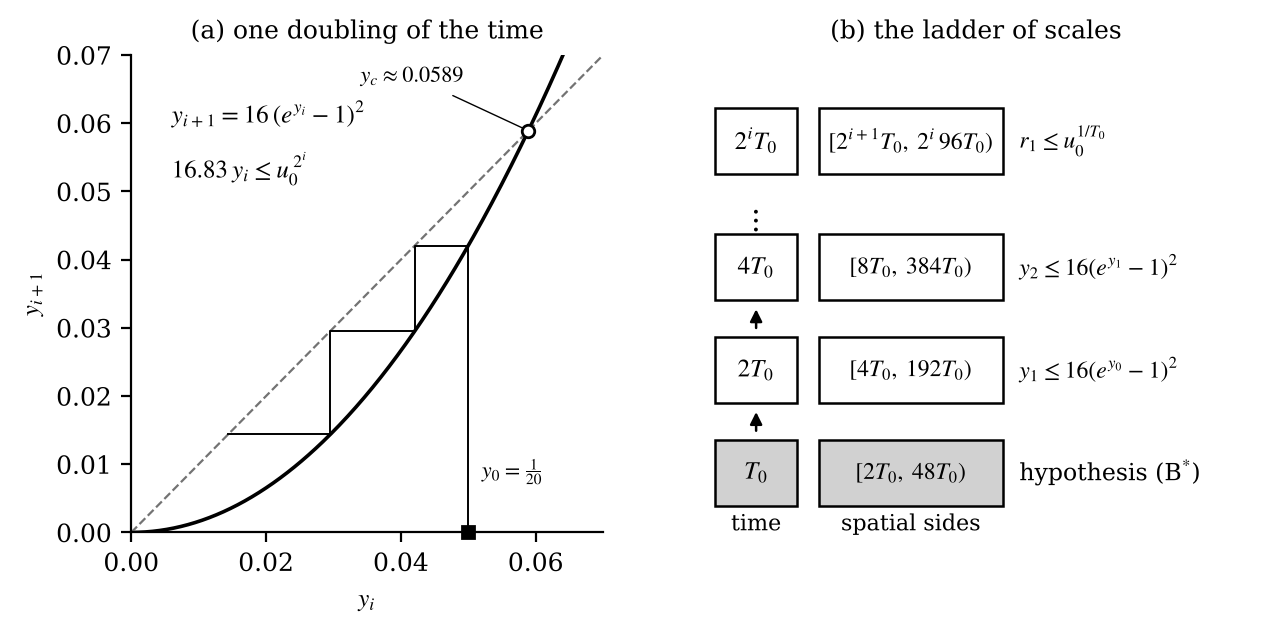
\includegraphics[width=\textwidth]{figures/fig_ascent.png}
\caption{The ascent of Theorem~\ref{thm:ascentfree}. (a) One doubling of the time extent maps the normalised pressure $y_i$ to at most $16(e^{y_i}-1)^2$; below the fixed point $y_c$ the iteration decreases doubly exponentially, and the starting value $y_0\le\frac1{20}$ lies below it. (b) The hypothesis is made at the single time extent $T_0$ (grey); every larger scale, with its gap, is a consequence.}
\label{fig:ascent}
\end{figure}

\begin{mainthmF}[the mass gap from one scale]\label{thm:F}
Let a continuum family satisfy \textup{(W)}, and suppose there are $t_0>0$,
$y_0\le\frac1{20}$ and $p_0$, $N_0(p)$ such that for all $p\ge p_0$ and $N\ge
N_0(p)$ there is an integer $T_0$ with $3\le T_0\le Nt_0$ for which
\textup{(B$^*$)} holds at the coupling $\beta_{N,p}$ with $\gamma=y_0/(2(96
T_0)^3)$. Put $u_0=16.83\,y_0$ and
\[
\Delta=\frac{\log(1/u_0)}{t_0}\ge\frac{0.172}{t_0} .
\]
Then, for $L_p\ge2t_0$:
\begin{enumerate}[label=\textup{(\roman*)},leftmargin=*]
\item $\mathcal Z_{N,p}-1\le1.9\cdot10^{-11}e^{-\Delta L_p/2}$, so the family
satisfies \textup{(Z)};
\item every eigenvalue $\lambda\ne\lambda_0$ of the transfer matrix of the
cylinder of spatial side $NL_p$ satisfies $0\le\lambda\le e^{-\Delta/N}
\lambda_0$;
\item the conclusion of Theorem~\ref{thm:E} holds with this $\Delta$: $S^\chi$
does not depend on $\chi$, and the Wightman theory of \textup{(W)} has
$\sigma(H)\subset\{0\}\cup[\Delta,\infty)$ with $0$ a simple eigenvalue.
\end{enumerate}
Neither \textup{(U)}, nor \textup{(D$_\ell$)}, nor the slab hypothesis
\textup{(M)}, nor \textup{(G$_{24}$)} is assumed.
\end{mainthmF}

\begin{proof}
Put $n=NL_p$; then $n\ge2Nt_0\ge2T_0$. (i) is
Theorem~\ref{thm:ascentfree}(c), with $u_0^{\,n/(2T_0)}\le u_0^{L_p/(2t_0)}=
e^{-\Delta L_p/2}$ because $T_0\le Nt_0$ and $u_0<1$; and $L_p\to\infty$.
(ii) is Theorem~\ref{thm:ascentfree}(b) for the cube of side $n$: $r_1\le
u_0^{1/T_0}\le u_0^{1/(Nt_0)}=e^{-\Delta/N}$, the eigenvalues being
nonnegative by Lemma~\ref{lem:transfer}(vii). (iii) In Step~1 of
Section~\ref{ssec:assembly}, hypothesis (D$_\ell$) enters only through
Proposition~\ref{prop:cylindergap}, which gives the transfer matrix of the
cylinder of side $NL_p$ a gap $m$ with $mN\ge\Delta$, and
Lemma~\ref{lem:gaptodecay} then gives~\eqref{eq:latticeineq} with the factor
$e^{-mN(\sigma-\sigma_1)}\le e^{-\Delta(\sigma-\sigma_1)}$. Here (ii) is that
gap, with $m=\Delta/N$, so~\eqref{eq:latticeineq} holds with the factor
$e^{-\Delta(\sigma-\sigma_1)}$. By (i) and Proposition~\ref{prop:ZgivesU},
\textup{(W)} gives \textup{(U$_w$)}, and the proof of
Corollary~\ref{cor:Z} derives~\eqref{eq:limitineq} from~\eqref{eq:latticeineq}
and \textup{(U$_w$)}, using the gap only through that factor. Steps~3
and~4 use~\eqref{eq:limitineq} and \textup{(W)} alone.
\end{proof}

Theorem~F replaces the hypotheses (D$_\ell$) or (M), (G$_{24}$), (Z) and (U)
by one bound at one scale. That bound does not involve the side $L_p$, an
insertion or a renormalisation constant, and it has a finite form.

\begin{proposition}[finite form]\label{prop:Bfinite}
With $\psi_s(T)=2\log Z(s,T)-\log Z(s,2T)$ as in Section~\ref{ssec:onescale},
hypothesis \textup{(B$^*$)} with the constant $\gamma$ follows from
\[
\textup{(B$^{**}$)}\qquad Z(s,T_0)^2\le e^{\gamma V(s)}\,Z(s,2T_0)\qquad
\text{for every }s\text{ with all its sides in }[2T_0,48T_0),
\]
and \textup{(B$^*$)} with $\gamma$ implies \textup{(B$^{**}$)} with $2\gamma$.
\textup{(B$^{**}$)} compares the partition functions of $2\cdot(46T_0)^3$
finite four-dimensional tori and is unchanged when $Z(n)$ is multiplied by
$e^{a|n|}$.
\end{proposition}

\begin{proof}
Lemma~\ref{lem:doubling} for the time transfer matrix of $s$ gives $\log
\mathcal Z_s(T_0)\le\psi_s(T_0)\le2\log\mathcal Z_s(T_0)$, and (B$^{**}$) is
$\psi_s(T_0)\le\gamma V(s)$.
\end{proof}

With $\rho=\mathbb R^{T_0}/\Tr\mathbb R^{T_0}$, the thermal state of the
torus $s$ at the time extent $T_0$, the ratio $Z(s,2T_0)/Z(s,T_0)^2$ is
$\Tr\rho^2$, so (B$^{**}$) says that this state is nearly pure: $\Tr\rho^2\ge
e^{-\gamma V(s)}$. In physical terms (B$^{**}$) asks that the thermal part of the free energy
at the temperature $1/t_0$, in boxes of sides between $2t_0$ and $48t_0$, be
at most $y_0/(2\cdot96^3t_0^3)\le2.9\cdot10^{-8}\,t_0^{-3}$ per unit volume.
Two results delimit what a proof of it must contain.

\begin{proposition}[\textup{(B$^*$)} contains the lattice mass gap]
\label{prop:Bhard}
Suppose \textup{(B$^*$)} holds at a coupling $\beta$ for some $T_0$, and let
$\mu^0_n$ be the zero-temperature state of the cylinder of spatial side $n$.
Then for every $n\ge2T_0$, every bounded measurable function $F$ of a slab
$[0,w]$ and every integer $s\ge0$,
\[
0\le\mu^0_n(\vartheta\bar F\,\tau_sF)-|\mu^0_n(F)|^2\le\|F\|_\infty^2\,
e^{-\delta_*s},\qquad\delta_*=\frac{\log(1/u_0)}{T_0},
\]
and the same bound holds, for local $F$, for every weak-$*$ limit point of
$(\mu^0_n)_n$ on $\Z^3\times\Z$.
\end{proposition}

\begin{proof}
By Lemma~\ref{lem:transfer}(v) the middle term is $\ip{\Psi'_F}{\mathbb R^s
\Psi'_F}$ with $\Psi'_F\perp\Omega_0$. By Theorem~\ref{thm:ascentfree}(b),
$0\le\mathbb R\le e^{-\delta_*}$ on $\Omega_0^\perp$, and $\|\Psi'_F\|^2\le
\|\Psi_F\|^2=\mu^0_n(\vartheta\bar F\,F)\le\|F\|_\infty^2$. The bound is
uniform in $n$, so it passes to limit points.
\end{proof}

A proof of (B$^*$) along couplings $\beta\to\infty$ therefore proves
exponential clustering of four-dimensional lattice Yang--Mills theory at
arbitrarily weak coupling, with a rate $\log(1/u_0)/T_0(\beta)$. The base
scale $T_0(\beta)$ cannot stay bounded, by the next theorem: at a fixed
lattice size the gap closes as $\beta\to\infty$. We state it for $\SU(2)$,
where the weight of Section~\ref{sec:lattice} is $\exp(c\sum_p\ReTr Q_p)$
with $c=2\beta$.

\begin{theorem}[the gap closes at a fixed lattice size]\label{thm:gapcloses}
Let $G=\SU(2)$, $c=2\beta\ge\frac1{32}$ and
\[
\varepsilon(c)=\frac{12(\log c+5.42)}{c} .
\]
For every spatial torus $t=(\ell_1,\ell_2,\ell_3)$ with sides at least $3$
and $(\ell_1\ell_2)^2\varepsilon(c)<3$,
\[
1-r_1(t)\le\frac{2(\ell_1+\ell_2)^2\,\varepsilon(c)}{1-(\ell_1\ell_2)^2
\varepsilon(c)/3} .
\]
\end{theorem}

\begin{proof}
Write $A_p=2-\Tr Q_p=\frac12\|Q_p-1\|_F^2\in[0,4]$, with the Frobenius norm,
since $\|U-1\|_F^2=4-2\Tr U$ for $U\in\SU(2)$.

\emph{Step 1: an energy bound uniform in the torus.} On a torus with $|n|$
sites, $4|n|$ links and $6|n|$ plaquettes let $A=\sum_pA_p$ and $\tilde Z(c)=
\int e^{-cA}\prod_edQ_e\le1$, so that the Wilson measure is $\tilde Z(c)^{-1}
e^{-cA}\prod_edQ_e$ and $\E_c[A]=-(\log\tilde Z)'(c)$. Since $(\log\tilde
Z)''=\Var_c(A)\ge0$, the mean $\E_c[A]$ is nonincreasing in $c$, and
\[
\frac c2\,\E_c[A]\le\int_{c/2}^c\E_{c'}[A]\,dc'=\log\tilde Z(c/2)-\log\tilde
Z(c)\le-\log\tilde Z(c).
\]
If every link has $\|Q_e-1\|_F\le r$, then $\|Q_p-1\|_F\le4r$ and $A_p\le8r^2$.
In the class angle $\theta\in[0,\pi]$, with $\Tr U=2\cos\theta$, Haar
measure is $\frac2\pi\sin^2\theta\,d\theta$ and $\|U-1\|_F=\sqrt8\sin(\theta/
2)$. The ball of radius $r\le2$ is $\{\theta\le\theta_r\}$ with $\theta_r=2
\arcsin(r/\sqrt8)\in[r/\sqrt2,\pi/2]$, and by $\sin\theta\ge2\theta/\pi$ on
$[0,\pi/2]$ its measure is at least $\frac2\pi\int_0^{\theta_r}(2\theta/\pi)^2
d\theta=8\theta_r^3/(3\pi^3)\ge2\sqrt2\,r^3/(3\pi^3)\ge r^3/33$. With $r^2=1/
(8c)$, which has $r\le2$ because $c\ge\frac1{32}$, restricting the integral
to these balls gives $\tilde Z(c)\ge e^{-6|n|}(r^3/33)^{4|n|}$, so
\[
\E_c[A]\le\frac2c\,|n|\bigl(6+4\log33+6\log(8c)\bigr)\le\frac{12}c\,|n|\,
(\log c+5.42).
\]
The $|n|$ translates of a plaquette have equal expectation and $A_p\ge0$,
so $\E_c[A_p]\le\varepsilon(c)$ for every plaquette on every torus, and by
Lemma~\ref{lem:transfer}(v) the same bound holds for $\mu^0_t=\lim_M\mu_{t,M}$.

\emph{Step 2: three slice functions of mean zero.} On the slice at time $0$
let $P_1$ and $P_2$ be the ordered products of the links from the origin
once around the directions $1$ and $2$, and $F_1=\Tr P_1$, $F_2=\Tr P_2$,
$F_3=\Tr(P_1P_2)$; they are real, continuous and gauge invariant, being
traces of closed loops. The centre flip $z_1$, which replaces $Q_{(x,1)}$ by
$-Q_{(x,1)}$ on all links in the direction $1$ with $x_1=0$, at all times,
preserves Haar measure and every plaquette variable, because the two links
in the direction $1$ of a plaquette have the same coordinate $x_1$, so a
plaquette contains none or two of the flipped links. It therefore preserves
$\mu_{t,M}$ and $\mu^0_t$, and it maps $F_1$ to $-F_1$ and $F_3$ to $-F_3$.
The flip $z_2$ maps $F_2$ to $-F_2$. So $\mu^0_t(F_k)=0$ for $k=1,2,3$, that
is, $F_k\Omega_0\perp\Omega_0$.

\emph{Step 3: the three functions are not all small.} For $A,B\in\SU(2)$
with $x=\Tr A$, $y=\Tr B$ and $z=\Tr AB$, Fricke's identity is
\[
\Tr(ABA^{-1}B^{-1})=x^2+y^2+z^2-xyz-2 ;
\]
it follows from $\Tr(AB)+\Tr(AB^{-1})=xy$, applied three times.\footnote{The
Cayley--Hamilton identity $B+B^{-1}=y\cdot1$ gives $\Tr(AB)+\Tr(AB^{-1})=xy$
for $A,B\in\SU(2)$. Hence $\Tr(ABA^{-1}B^{-1})=\Tr(AB)\Tr(A^{-1}B^{-1})-
\Tr(ABBA)$, $\Tr(A^{-1}B^{-1})=\Tr(BA)=z$, and $\Tr(ABBA)=\Tr(A^2B^2)=\Tr(A^2B)
y-\Tr(A^2)$, with $\Tr(A^2B)=xz-y$ and $\Tr(A^2)=x^2-2$; so the commutator has
trace $z^2-(xz-y)y+x^2-2$.} Put $\sigma=x^2+y^2+z^2$ and $\eta=2-\Tr(ABA^{-1}
B^{-1})\ge0$. Since $|xyz|\le(\sigma/3)^{3/2}$, the function $\phi(\sigma)=
\sigma+(\sigma/3)^{3/2}$ satisfies $\phi(\sigma)\ge4-\eta$. As $\phi(3)=4$ and
$\phi'\ge1$, $\sigma<3$ gives $3-\sigma\le\phi(3)-\phi(\sigma)\le\eta$; so
$\sigma\ge3-\eta$ in every case. Apply this to $A=P_1$ and $B=P_2$. The
commutator $K=P_1P_2P_1^{-1}P_2^{-1}$ is the holonomy of the boundary of the
sheet of the $\ell_1\ell_2$ plaquettes of the $(1,2)$-plane through the
origin, cut open along the two cycles. Adding the plaquettes of the sheet
one at a time, row by row, so that each step keeps a disc, multiplies the
boundary holonomy by a conjugate of $Q_p^{\pm1}$; so $K$ is a product of
$\ell_1\ell_2$ conjugates of the $Q_p^{\pm1}$, and $\|UV-1\|_F\le\|U-1\|_F+
\|V-1\|_F$ for unitary matrices gives $\|K-1\|_F\le\sum_p\|Q_p-1\|_F$.
Hence, by the Cauchy--Schwarz inequality,
\[
\eta=\tfrac12\|K-1\|_F^2\le\tfrac12\Bigl(\sum_p\sqrt{2A_p}\Bigr)^2\le\ell_1
\ell_2\sum_{p}A_p,\qquad\mu^0_t(\eta)\le(\ell_1\ell_2)^2\varepsilon ,
\]
the sums over the plaquettes of the sheet. So $\sum_k\mu^0_t(F_k^2)\ge3-(\ell_1
\ell_2)^2\varepsilon$, and some $k$ has $\|F_k\Omega_0\|^2=\mu^0_t(F_k^2)\ge1-
(\ell_1\ell_2)^2\varepsilon/3$.

\emph{Step 4: the Dirichlet form.} For a real function $F$ of the slice,
Lemma~\ref{lem:transfer}(v) with $w=w'=0$ and $s=1$, and the invariance of
$\mu^0_t$ under time translations, give
\[
\ip{F\Omega_0}{(1-\mathbb R)F\Omega_0}=\mu^0_t(F^2)-\mu^0_t(F\,\tau_1F)=\tfrac
12\,\mu^0_t\bigl((F-\tau_1F)^2\bigr).
\]
The loop of $F_k$ at time $0$ and its translate at time $1$, joined by the
temporal link at the origin, bound a strip of $m_k$ temporal plaquettes,
with $m_1=\ell_1$, $m_2=\ell_2$ and $m_3=\ell_1+\ell_2$. As in Step~3 the two
holonomies $X$ and $Y$, the second conjugated by the temporal link, satisfy
$\|X-Y\|_F\le\sum_p\|Q_p-1\|_F$ over the strip, and $|\Tr X-\Tr Y|\le\sqrt2\,
\|X-Y\|_F$. So $(F_k-\tau_1F_k)^2\le4m_k\sum_pA_p$ and
\[
\tfrac12\,\mu^0_t\bigl((F_k-\tau_1F_k)^2\bigr)\le2m_k^2\,\varepsilon\le2(\ell_1+
\ell_2)^2\varepsilon .
\]

\emph{Step 5.} On $\Omega_0^\perp$ one has $\mathbb R\le r_1$, so for the $k$
of Step~3, $1-r_1\le\ip{F_k\Omega_0}{(1-\mathbb R)F_k\Omega_0}/\|F_k\Omega_0\|^2$,
which is the claim.
\end{proof}

\begin{corollary}[the base scale diverges]\label{cor:basescale}
If \textup{(B$^*$)} holds for $\SU(2)$ with the base scale $T_0$ at a
coupling with $\varepsilon=\varepsilon(2\beta)\le10^{-3}$, then
\[
T_0>\Bigl(\frac3{32\,\varepsilon}\Bigr)^{1/4}=\Bigl(\frac{\beta}{64(\log2\beta
+5.42)}\Bigr)^{1/4}.
\]
\end{corollary}

\begin{proof}
On the cube $t$ of side $2T_0$, (B$^*$) gives $r_1^{T_0}\le D_t(T_0)\le e^{8
\gamma T_0^3}-1=e^{4y_0/96^3}-1\le2.3\cdot10^{-7}$, so $r_1\le e^{-x}$ with $x=
15.28/T_0$, and by concavity $1-r_1\ge(1-e^{-1})\min\{1,x\}\ge\min\{0.632,\,
9.6/T_0\}$. Suppose $T_0^4\varepsilon\le\frac3{32}$. Then $(2T_0)^4\varepsilon
\le\frac32$, and Theorem~\ref{thm:gapcloses} with $\ell_1=\ell_2=2T_0$ gives
$1-r_1\le64T_0^2\varepsilon$. If $T_0\le15$ this is at most $64\sqrt{3/32}\,
\sqrt\varepsilon\le0.62<0.632$, and if $T_0\ge16$ it gives $T_0^3\varepsilon
\ge0.15$, while $T_0^3\varepsilon\le\frac3{32\cdot16}<0.006$. Both are
impossible.
\end{proof}

Thus no tuning with $\beta_N\to\infty$ has its base scale at a bounded
number of lattice units, and a bound of the shape of
Proposition~\ref{prop:Zstrongsharp}, with a rate fixed in lattice units,
cannot serve along it (Proposition~\ref{prop:nofixedrate}); the mechanism
is the centre symmetry, which gives the Polyakov loops mean zero while the
action no longer suppresses their fluctuation at a fixed lattice size. The
proof of Theorem~\ref{thm:ascentfree} uses of the Wilson action only that
$Z$ is symmetric in the four sides and is, in each direction, the trace of
a power of a nonnegative self-adjoint Hilbert--Schmidt operator with a
simple largest eigenvalue.
What remains open for four-dimensional Yang--Mills theory at weak coupling
is therefore (W) and the one bound \textup{(B$^{**}$)}, for integers $T_0
(\beta)\to\infty$ along a sequence $\beta\to\infty$:
\[
Z(s,T_0)^2\le\exp\Bigl(\frac{V(s)}{40\,(96T_0)^3}\Bigr)Z(s,2T_0)\qquad
\text{for every }s\text{ with all its sides in }[2T_0,48T_0).
\]
Neither is proved here.
